\documentclass[11pt, a4paper]{article}

\usepackage[a4paper, margin=2.5cm]{geometry}
\usepackage{amsmath}
\usepackage{booktabs}
\usepackage{tabularx}
\usepackage[table]{xcolor}
\usepackage{hyperref}
\usepackage{graphicx}

\definecolor{isiBlue}{RGB}{20, 50, 100}
\definecolor{flowBg1}{RGB}{225, 238, 250}
\definecolor{flowBg2}{RGB}{222, 244, 230}
\definecolor{flowBg3}{RGB}{254, 240, 217}
\definecolor{flowBg4}{RGB}{242, 229, 250}

\hypersetup{
    colorlinks=true,
    linkcolor=isiBlue,
    urlcolor=isiBlue,
    citecolor=isiBlue
}

\setlength{\parindent}{0pt}
\setlength{\parskip}{6pt}

\begin{document}

\begin{titlepage}
    \centering
    \vspace*{1.5cm}
    
    %{\Large \textbf{\{AUTUMN INTERNSHIP PROJECT REPORT FORMAT\}}} \\[2.2cm]
    
    {\LARGE \textbf{Project 1: Predicting India's GDP Growth with Simple Regressions}} \\[2.2cm]
    
    {\Large \textbf{Debodirna Ghosh}} \\[0.3cm]
    %{\large \textbf{Group Members: Arpan Das, Debodirna Ghosh and Renu Parashar}} \\[0.4cm]
    {\large \textbf{[Course/batch and Institute name]}} \\[2cm]
    
    {\large \textbf{Period of Internship: 21st September 2026 -- 30th November 2026}} \\[2.2cm]
    
    {\Large \textbf{Report submitted to: IDEAS -- Institute of Data}} \\[0.2cm]
    {\Large \textbf{Engineering, Analytics and Science Foundation, ISI}} \\[0.2cm]
    {\Large \textbf{Kolkata}} \\[2.5cm]
    
    {\large \textbf{Project Mentor: $<$Mentor Name$>$}}
    
    \vfill
\end{titlepage}

\section{Abstract}
Official quarterly GDP estimates for India are published roughly two months after the quarter ends, whereas several monthly indicators become available much sooner. This project tests whether three such indicators, the Index of Industrial Production (IIP), merchandise exports in US dollars and non-food bank credit, can estimate current-quarter real GDP growth before the official release. Every series was converted to a quarterly average and then to year-on-year (YoY) growth, which removes the need for seasonal adjustment. Three single-indicator regressions and one multiple regression were estimated by ordinary least squares (OLS) on 32 quarters from FY2012-13 to FY2019-20. They were then tested on 14 quarters from FY2022-23 to Q2 FY2025-26 against a naive benchmark that repeats the previous quarter's growth. IIP was the only indicator with a statistically significant relationship with GDP growth ($R^2 = 0.30$, $p = 0.001$). The IIP regression also gave the lowest test errors (MAE 1.25 and RMSE 1.53 percentage points, against 2.11 and 3.37 for the naive benchmark). The multiple regression was nearly as accurate (MAE 1.26, RMSE 1.60) but did not improve on IIP alone. Exports and credit had no significant explanatory power by themselves. A simple IIP-based regression is therefore a useful and transparent nowcasting tool for India's GDP growth.

\section{Introduction}
GDP is the broadest measure of economic activity, but the official quarterly figure arrives with a lag of about two months. Policymakers, businesses and investors often need an estimate of current growth before then. Estimating the current quarter from indicators that are already published is called nowcasting. A common and simple approach, used by many central banks and research institutions, is a bridge regression that links GDP growth to a small set of higher-frequency indicators.

This project builds such regressions for India using three monthly indicators. The IIP General Index measures output of mining, manufacturing and electricity and is closely tied to the industrial part of GDP. Merchandise exports in US dollars capture external demand. Non-food bank credit of scheduled commercial banks reflects financing conditions and domestic demand. All three are released well before GDP and are freely available from official sources.

The work was done in Python using \texttt{pandas} for data handling, \texttt{statsmodels} for OLS estimation and \texttt{matplotlib} for charts. The procedure was to download and clean the data, convert each series to quarterly YoY growth, plot each indicator against GDP growth, split the sample into training and test periods, fit the regressions on the training period, and compare their test-period forecasts with a naive benchmark using MAE and RMSE. The purpose is both to learn the practical workflow of an applied forecasting problem and to answer a concrete question: does a simple indicator-based model beat a naive guess?

\textbf{Topics covered in the training during the first two weeks of the internship:} [Add the list of topics here].

\section{Project Objective}
The project has five objectives:
\begin{itemize}
    \item Build comparable quarterly YoY growth series for real GDP (2011-12 base) and the three indicators.
    \item Examine graphically how each indicator moves with GDP growth.
    \item Estimate three single regressions and one multiple regression by OLS on a pre-COVID training period (FY2012-13 to FY2019-20).
    \item Predict GDP growth for a test period (FY2022-23 to Q2 FY2025-26) and measure the errors with MAE and RMSE.
    \item Test whether the regression models beat the naive benchmark, in which this quarter's growth equals last quarter's growth.
\end{itemize}

\textbf{Hypotheses tested.} For each indicator the null hypothesis is that its slope coefficient is zero (no linear relationship with GDP growth), against the alternative that it is not zero, using a $t$-test at the 5\% level. For the multiple regression the joint null hypothesis is that all three slopes are zero, using an $F$-test. The forecasting hypothesis is that each regression has lower MAE and RMSE than the naive benchmark on the test quarters. No sample survey was conducted; all data are official published statistics.

\section{Methodology}

\subsection{Data sources}
\begin{table}[h!]
\centering
\small
\renewcommand{\arraystretch}{1.3}
\begin{tabularx}{\textwidth}{>{\raggedright\arraybackslash}p{4.0cm} >{\raggedright\arraybackslash}p{3.4cm} l >{\raggedright\arraybackslash}X}
\toprule
\textbf{Series} & \textbf{Source} & \textbf{Frequency} & \textbf{Coverage used} \\
\midrule
Real GDP at constant prices (2011-12 base) & RBI DBIE (MoSPI national accounts) & Quarterly & Q1 FY2011-12 to Q2 FY2025-26 \\
IIP General Index (base 2011-12) & MoSPI eSankhyiki & Monthly & April 2012 to March 2026 \\
Merchandise exports, oil plus non-oil (US\$) & RBI DBIE & Monthly & Full series downloaded; modelling uses data to September 2025 \\
Non-food bank credit of scheduled commercial banks & RBI DBIE & Fortnightly & Full series downloaded; modelling uses data to September 2025 \\
\bottomrule
\end{tabularx}
\caption{Summary of data sources and coverage}
\end{table}

Indian fiscal quarters are used throughout: Q1 is April--June, Q2 is July--September, Q3 is October--December and Q4 is January--March. Each quarter is identified by its end date.

\subsection{Data cleaning and pre-processing}
\textbf{GDP.} The quarterly series was sorted by date and YoY growth was computed as:
\[
\text{Growth}_t = \left(\frac{\text{GDP}_t}{\text{GDP}_{t-4}} - 1\right) \times 100
\]
The first growth value is therefore Q1 FY2012-13.

\textbf{IIP.} The two downloaded IIP files were combined, the year and month name were converted to dates, and the data were sorted. The twelve months of the base year 2011-12 were added with an index of 100 so that YoY growth could be computed for FY2012-13. Each quarter's value is the average of its three monthly indices.

\textbf{Exports.} Oil and non-oil exports were added to get total merchandise exports. The financial year and month name were converted to calendar dates, and the monthly values were averaged by quarter.

\textbf{Non-food credit.} Header and footer rows were removed, Indian-style digit grouping (for example 2,29,94,852) was stripped and values were converted to numbers. Missing and non-positive entries were dropped, because an early run that kept them produced implausible recent growth rates (for example $-52.9\%$ and $-80.6\%$). The remaining fortnightly observations were averaged by quarter.

For every indicator, YoY growth was calculated from the quarterly average in the same way as for GDP. The four growth series were merged on the quarter-end date and restricted to Q1 FY2012-13 to Q2 FY2025-26, giving 54 quarterly observations. The cleaned series were also exported to Excel files.

\subsection{Train-test split}
The split is chronological, with no shuffling.

\begin{table}[h!]
\centering
\renewcommand{\arraystretch}{1.2}
\begin{tabular}{l l c}
\toprule
\textbf{Period} & \textbf{Quarters} & \textbf{Number of quarters} \\
\midrule
Training & Q1 FY2012-13 to Q4 FY2019-20 & 32 \\
Excluded & FY2020-21 and FY2021-22 & 8 \\
Test & Q1 FY2022-23 to Q2 FY2025-26 & 14 \\
\bottomrule
\end{tabular}
\caption{Chronological train-test split of the quarterly sample}
\end{table}

FY2020-21 and FY2021-22 are left out of both samples because the COVID-19 shock produced extreme growth rates (from $-23.1\%$ to $+22.6\%$) that would dominate estimation and are not representative of normal conditions.

\subsection{Models and benchmark}
Let $Y_t$ denote the quarterly YoY real GDP growth rate at quarter $t$, and let $X_{1,t}$, $X_{2,t}$, and $X_{3,t}$ denote the quarterly YoY growth rates of the IIP General Index, Merchandise Exports (in US\$), and Non-Food Bank Credit, respectively. Four linear regression models were estimated by Ordinary Least Squares (OLS) using \texttt{statsmodels} on the training period:
\begin{align}
    \textbf{Model 1 (Single OLS -- IIP):} \quad Y_t &= \beta_0 + \beta_1 X_{1,t} + \varepsilon_t \\
    \textbf{Model 2 (Single OLS -- Exports):} \quad Y_t &= \beta_0 + \beta_1 X_{2,t} + \varepsilon_t \\
    \textbf{Model 3 (Single OLS -- Credit):} \quad Y_t &= \beta_0 + \beta_1 X_{3,t} + \varepsilon_t \\
    \textbf{Model 4 (Multiple OLS -- All 3):} \quad Y_t &= \beta_0 + \beta_1 X_{1,t} + \beta_2 X_{2,t} + \beta_3 X_{3,t} + \varepsilon_t
\end{align}
where $\beta_0$ is the intercept, $\beta_i$ ($i = 1, 2, 3$) are the slope coefficients, and $\varepsilon_t$ is the error term.

The naive benchmark predicts that the current quarter's GDP growth equals the previous quarter's GDP growth:
\[
\hat{Y}_t^{\text{naive}} = Y_{t-1}
\]
Model selection was kept deliberately simple, as the aim was to compare the indicators fairly, so each model was fitted once on the training data and not tuned using the test data.

\subsection{Evaluation}
Each fitted model was used to predict GDP growth for the 14 test quarters from the indicator values of the same quarter. Accuracy was measured by the mean absolute error (MAE) and the root mean squared error (RMSE), both in percentage points. RMSE penalises large misses more heavily than MAE.

Figure 1 summarises the workflow. The Python notebook is available at the GitHub link given in Appendix 3.

\begin{figure}[h!]
\centering
\renewcommand{\arraystretch}{1.7}
\setlength{\tabcolsep}{4pt}
\begin{tabular}{|>{\columncolor{flowBg1}\centering\arraybackslash}p{3.2cm}|c|>{\columncolor{flowBg1}\centering\arraybackslash}p{3.2cm}|c|>{\columncolor{flowBg2}\centering\arraybackslash}p{3.2cm}|c|>{\columncolor{flowBg2}\centering\arraybackslash}p{3.2cm}|}
\cline{1-1}\cline{3-3}\cline{5-5}\cline{7-7}
\small \textbf{\textcolor{isiBlue}{1. Data Collection}}\newline Download GDP, IIP, exports, credit & \textcolor{isiBlue}{$\boldsymbol{\rightarrow}$} &
\small \textbf{\textcolor{isiBlue}{2. Pre-processing}}\newline Clean dates, units \& missing values & \textcolor{isiBlue}{$\boldsymbol{\rightarrow}$} &
\small \textbf{\textcolor{isiBlue}{3. Aggregation}}\newline Quarterly averages of high-freq series & \textcolor{isiBlue}{$\boldsymbol{\rightarrow}$} &
\small \textbf{\textcolor{isiBlue}{4. Transformation}}\newline Compute YoY growth rates (\%) \\
\cline{1-1}\cline{3-3}\cline{5-5}\cline{7-7}
\multicolumn{6}{c}{} & \multicolumn{1}{c}{\textcolor{isiBlue}{$\boldsymbol{\downarrow}$}} \\
\cline{1-1}\cline{3-3}\cline{5-5}\cline{7-7}
\multicolumn{1}{|>{\columncolor{flowBg4}\centering\arraybackslash}p{3.2cm}|}{\small \textbf{\textcolor{isiBlue}{8. Evaluation}}\newline Predict test qtrs; MAE \& RMSE vs naive} & \textcolor{isiBlue}{$\boldsymbol{\leftarrow}$} &
\multicolumn{1}{>{\columncolor{flowBg4}\centering\arraybackslash}p{3.2cm}|}{\small \textbf{\textcolor{isiBlue}{7. OLS Estimation}}\newline Fit 3 single \& 1 multiple model} & \textcolor{isiBlue}{$\boldsymbol{\leftarrow}$} &
\multicolumn{1}{>{\columncolor{flowBg3}\centering\arraybackslash}p{3.2cm}|}{\small \textbf{\textcolor{isiBlue}{6. Sample Split}}\newline Train: 32 / Test: 14 (COVID excluded)} & \textcolor{isiBlue}{$\boldsymbol{\leftarrow}$} &
\multicolumn{1}{>{\columncolor{flowBg3}\centering\arraybackslash}p{3.2cm}|}{\small \textbf{\textcolor{isiBlue}{5. Data Alignment}}\newline Merge on quarter-end (54 qtrs)} \\
\cline{1-1}\cline{3-3}\cline{5-5}\cline{7-7}
\end{tabular}
\caption{Scientific workflow of the GDP nowcasting analysis}
\end{figure}

\section{Data Analysis and Results}

\subsection{Descriptive analysis}
Figure 2 plots each indicator against real GDP growth. IIP growth tracks GDP growth closely, including the sharp fall in Q1 FY2020-21 and the rebound a year later. Export growth is far more volatile than GDP growth and swings widely around it, while non-food credit growth is smooth and slow-moving and often moves differently from GDP growth.

\begin{figure}[h!]
\centering
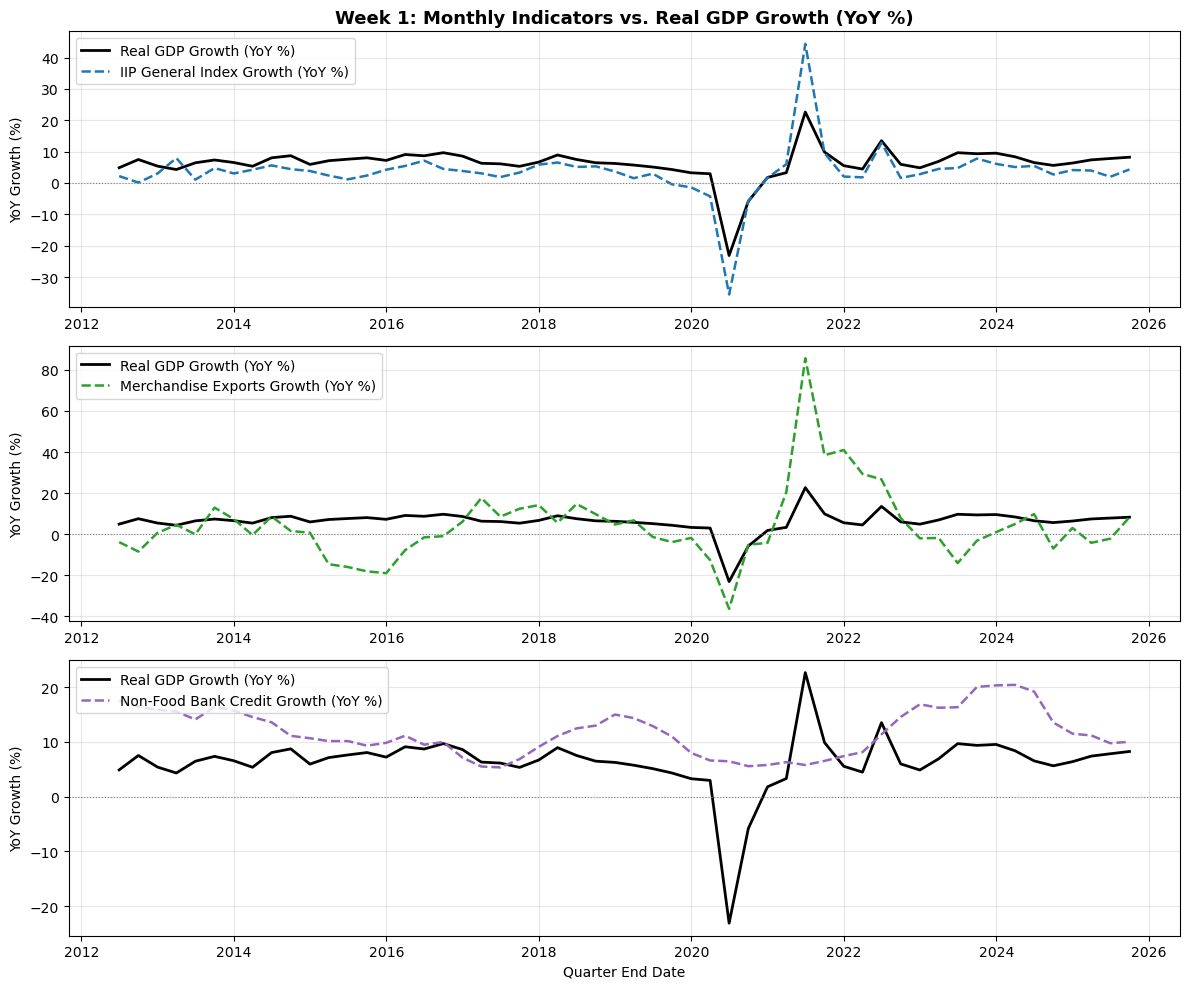
\includegraphics[width=0.92\textwidth]{fig2_indicators_vs_gdp.png}
\caption{Monthly indicators (quarterly average, YoY \%) against real GDP growth}
\end{figure}

\begin{table}[h!]
\centering
\renewcommand{\arraystretch}{1.2}
\begin{tabular}{l c c c c c}
\toprule
\textbf{GDP growth (YoY \%)} & \textbf{Quarters} & \textbf{Mean} & \textbf{Std. deviation} & \textbf{Minimum} & \textbf{Maximum} \\
\midrule
Training period & 32 & 6.60 & 1.69 & 2.94 & 9.67 \\
Test period & 14 & 7.86 & 2.21 & 4.84 & 13.49 \\
\bottomrule
\end{tabular}
\caption{Descriptive statistics of real GDP YoY growth (\%)}
\end{table}

Growth in the test period is higher on average and more variable than in the training period, which matters for the forecasting results below.

\subsection{Inferential analysis: regressions on the training period}

\begin{table}[h!]
\centering
\small
\renewcommand{\arraystretch}{1.35}
\setlength{\tabcolsep}{4pt}
\begin{tabularx}{\textwidth}{>{\raggedright\arraybackslash}p{2.9cm} c >{\raggedright\arraybackslash}p{2.4cm} >{\raggedright\arraybackslash}X c c c c}
\toprule
\textbf{Model} & \textbf{Intercept ($\hat{\beta}_0$)} & \textbf{Slope ($\hat{\beta}_i$)} & \textbf{$t$-stat ($p$-value)} & \textbf{$R^2$} & \textbf{Adj. $R^2$} & \textbf{$F$-test $p$-val} & \textbf{DW} \\
\midrule
1. Single: IIP ($X_1$) & $5.406$ & $\hat{\beta}_1 = 0.365$ & $3.58$ ($0.001$) & $0.299$ & $0.276$ & $0.001$ & $1.54$ \\
2. Single: Exports ($X_2$) & $6.599$ & $\hat{\beta}_1 = -0.002$ & $-0.06$ ($0.953$) & $0.000$ & $-0.033$ & $0.953$ & $0.70$ \\
3. Single: Credit ($X_3$) & $6.864$ & $\hat{\beta}_1 = -0.023$ & $-0.26$ ($0.800$) & $0.002$ & $-0.031$ & $0.800$ & $0.72$ \\
\addlinespace[4pt]
4. Multiple OLS & $6.108$ & $\hat{\beta}_1 = 0.466$\newline $\hat{\beta}_2 = -0.050$\newline $\hat{\beta}_3 = -0.086$ & $4.25$ ($<0.001$)\newline $-1.78$ ($0.085$)\newline $-1.15$ ($0.258$) & $0.393$ & $0.328$ & $0.003$ & $1.91$ \\
\bottomrule
\end{tabularx}
\caption{OLS regression estimates on the training period ($N = 32$, Q1 FY2012-13 to Q4 FY2019-20)}
\end{table}

With 32 observations, the IIP model is the only single regression in which the slope is significantly different from zero. A one percentage point rise in IIP growth is associated with about 0.37 percentage points higher GDP growth (95\% confidence interval 0.16 to 0.57). The export and credit slopes are close to zero with $p$-values above 0.8, so we cannot reject the null hypothesis for either, and their regressions are effectively just the training-period mean of GDP growth (about 6.6\%).

In the multiple regression the joint $F$-test is significant ($p = 0.003$) and $R^2$ rises to 0.393, but this is driven by IIP. IIP remains highly significant, exports are significant only at the 10\% level and credit is not significant. The negative signs on exports and credit run against economic intuition and should not be over-interpreted in a sample this small. Adjusted $R^2$ is higher for the multiple model (0.328 against 0.276), but BIC prefers the IIP-only model (118.9 against 121.2) and AIC is almost identical (116.0 against 115.4). The Jarque-Bera tests give no evidence against normal residuals ($p$-values from 0.28 to 0.72). The low Durbin-Watson values for the export and credit models (about 0.7) indicate strongly autocorrelated residuals, which is expected when a model only reproduces the mean of a persistent series.

\begin{figure}[h!]
\centering
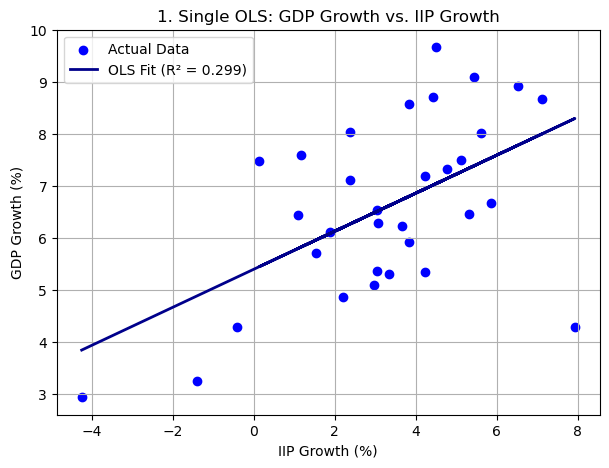
\includegraphics[width=0.32\textwidth]{fig3a_ols_iip.png}\hfill
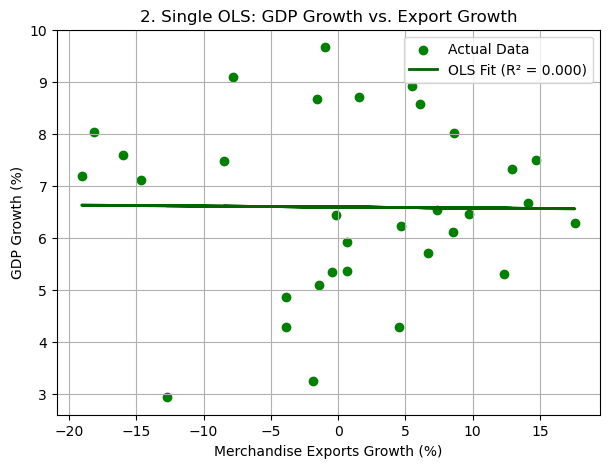
\includegraphics[width=0.32\textwidth]{fig3b_ols_exports.png}\hfill
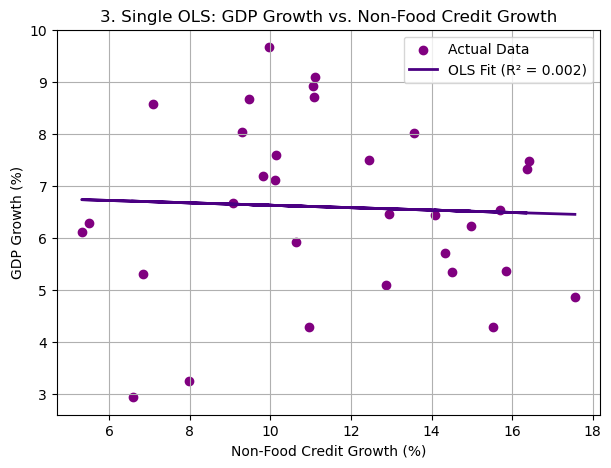
\includegraphics[width=0.32\textwidth]{fig3c_ols_credit.png}
\caption{Training period scatter plots with OLS fits (IIP, exports, non-food credit)}
\end{figure}

\begin{figure}[h!]
\centering
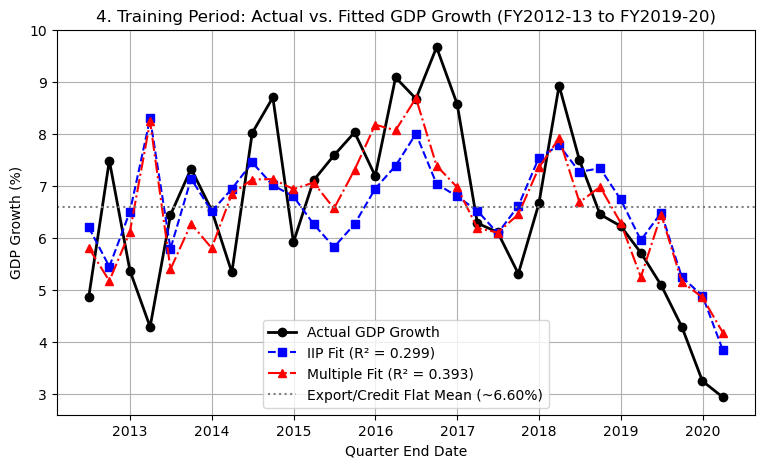
\includegraphics[width=0.82\textwidth]{fig4_train_actual_vs_fitted.png}
\caption{Training period, actual against fitted GDP growth}
\end{figure}


\subsection{Forecast evaluation on the test period}

\begin{table}[h!]
\centering
\small
\renewcommand{\arraystretch}{1.25}
\setlength{\tabcolsep}{5pt}
\begin{tabularx}{\textwidth}{>{\raggedright\arraybackslash}X c c >{\centering\arraybackslash}p{2.8cm} >{\centering\arraybackslash}p{2.8cm}}
\toprule
\textbf{Model} & \textbf{MAE (\%)} & \textbf{RMSE (\%)} & \textbf{MAE reduction vs naive} & \textbf{RMSE reduction vs naive} \\
\midrule
Naive benchmark ($\hat{Y}_t = Y_{t-1}$) & 2.1077 & 3.3717 & -- & -- \\
Single OLS: IIP ($X_1$) & 1.2462 & 1.5309 & 40.9\% & 54.6\% \\
Single OLS: Merchandise exports ($X_2$) & 1.7859 & 2.4773 & 15.3\% & 26.5\% \\
Single OLS: Non-food bank credit ($X_3$) & 1.8214 & 2.5124 & 13.6\% & 25.5\% \\
Multiple OLS: All three indicators & 1.2627 & 1.6002 & 40.1\% & 52.5\% \\
\bottomrule
\end{tabularx}
\caption{Out-of-sample forecast accuracy on the test period ($N = 14$, Q1 FY2022-23 to Q2 FY2025-26)}
\end{table}

All four regressions beat the naive benchmark on both measures. The IIP regression is the most accurate, cutting MAE by about 41\% and RMSE by about 55\%. The multiple regression is a close second but no better than IIP alone, which suggests that the extra two indicators add noise rather than information given only 32 training quarters.

The naive benchmark is weak mainly at turning points. About 87\% of its total squared error comes from the first two test quarters, when GDP growth jumped to 13.5\% in Q1 FY2022-23 and fell back to 6.0\% in Q2, so that repeating the previous quarter was badly wrong both times. The export and credit models are almost constant forecasts at about 6.6\%. A constant forecast equal to the training-period mean would have an MAE of 1.79 and an RMSE of 2.47, nearly the same as these two models, so their advantage over the naive benchmark reflects the naive rule's weakness rather than information in the indicators. Only IIP carries genuine predictive information.

Figure 5 shows actual and predicted growth over the test period. The regression forecasts are smoother than actual growth. They capture the high growth in Q1 FY2022-23 through IIP, but under-predict during FY2023-24 and the most recent three quarters, when GDP growth was higher than the 6.6\% average of the training period.

\begin{figure}[h!]
\centering
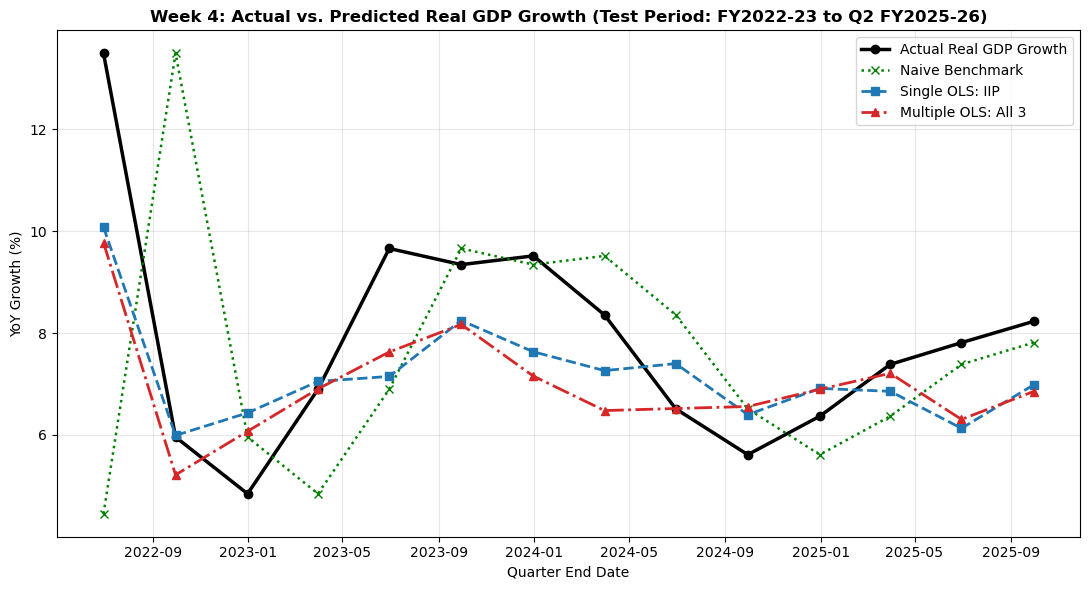
\includegraphics[width=0.88\textwidth]{fig5_test_actual_vs_pred.png}
\caption{Actual against predicted real GDP growth, test period (Q1 FY2022-23 to Q2 FY2025-26)}
\end{figure}

\section{Conclusion}
The project shows that a very simple model can estimate India's current-quarter GDP growth better than a naive guess. IIP growth explains about 30\% of the variation in GDP growth over FY2012-13 to FY2019-20, its slope is highly significant, and the resulting regression reduced test-period MAE from 2.11 to 1.25 and RMSE from 3.37 to 1.53 percentage points. Merchandise exports and non-food bank credit have no significant linear relationship with GDP growth on their own, and the multiple regression (MAE 1.26, RMSE 1.60) offers no gain over IIP alone. The best practical model from this exercise is therefore the single regression on IIP.

The results have limits. The training sample is small (32 quarters), the models are noticeably smooth and under-predicted the strong growth of FY2023-24 and the latest quarters, and the relationship estimated before COVID-19 may not hold unchanged afterwards. The 2011-12 months of the IIP were set to 100, which is only an approximation for the first four growth observations. Final revised data were used, not the data that would have been available in real time.

Future work could add further timely indicators such as GST collections, power demand or PMI, include lagged GDP growth and use robust standard errors to deal with autocorrelation, re-estimate the models on a rolling window that includes recent years, and evaluate forecasts on real-time data vintages.

\section{Appendices}

\subsection*{Appendix 1: References}
\begin{itemize}
    \item Ministry of Statistics and Programme Implementation (MoSPI), eSankhyiki portal: Index of Industrial Production (base 2011-12) and national accounts.
    \item Reserve Bank of India, Database on Indian Economy (DBIE), \url{https://data.rbi.org.in}: quarterly GDP, merchandise trade and bank credit statistics.
    \item Seabold, S. and Perktold, J. (2010). Statsmodels: Econometric and statistical modeling with Python. \textit{Proceedings of the 9th Python in Science Conference}.
    \item McKinney, W. (2010). Data structures for statistical computing in Python. \textit{Proceedings of the 9th Python in Science Conference}.
    \item Hunter, J. D. (2007). Matplotlib: A 2D graphics environment. \textit{Computing in Science \& Engineering}, 9(3), 90--95.
\end{itemize}

\subsection*{Appendix 2: Survey questionnaire}
Not applicable. No survey was conducted.

\subsection*{Appendix 3: GitHub link for the code}
[Add GitHub link to \texttt{GDP\_analysis.ipynb}]

\subsection*{Appendix 4: Other document links}
[Add links to the report, cleaned data files and presentation]

\end{document}